\documentclass[handout]{beamer}
\usetheme{metropolis}

\usepackage[spanish,activeacute]{babel}
\usepackage{amsmath, amssymb}
\usepackage{graphicx}
\usepackage{multirow}
\usepackage[ruled,vlined,lined]{algorithm2e}
\usepackage{fontspec}
\setsansfont{Lato}
\setmonofont{Inconsolata}

\newcommand{\factorial}{\ensuremath{\mbox{\sc Factorial}}}
\newcommand{\BIGOP}[1]{\mathop{\mathchoice%
{\raise-0.22em\hbox{\huge $#1$}}%
{\raise-0.05em\hbox{\Large $#1$}}{\hbox{\large $#1$}}{#1}}}
\newcommand{\bigtimes}{\BIGOP{\times}}
\vspace{-0.5cm}
\title{Procesamiento del Lenguaje Natural \\ Semántica vectorial}
\vspace{-0.5cm}
\author[Jorge Ortiz Fuentes]{Jorge Ortiz Fuentes}  
 

\date{\today}

\begin{document}
\begin{frame}
\titlepage
\end{frame}

\begin{frame}\frametitle{Motivación (1/2)}

  \begin{itemize}
   \item ¿Cómo recuperan documentos relevantes los motores de búsqueda como Duckduckgo o Google a partir de una consulta?
  \end{itemize}

Estos problemas se estudian en el campo de \emph{Information Retrieval}: la ciencia de la búsqueda de información en colecciones de documentos.

\end{frame}

\begin{frame}\frametitle{Motivación (2/2)}

¿Cómo puede una empresa procesar los reclamos que los usuarios dejan en sus portales web?

Estos problemas se estudian en los siguientes campos:

\begin{itemize}
 \item \emph{Text Mining}: extracción automática de conocimiento a partir de texto.
\end{itemize}

¡Ambos están estrechamente relacionados con el NLP! (las fronteras entre estos campos no son claras)

\end{frame}

\begin{frame}\frametitle{Tokenización}
  \begin{itemize}
   \item La tokenización es la tarea de dividir una oración o documento en piezas llamadas \emph{tokens}.
   \item Se pueden emplear transformaciones adicionales como la eliminación de caracteres especiales (puntuación), convertir a minúsculas, etc. \cite{manning2008}.
  \end{itemize}
  
  \begin{block}{Ejemplo}
    \centering
    \vspace{0.5em}
    Entrada:\\ 
    \texttt{Me gustan los perros y los gatos.}\\
    \vspace{0.5em}
    Tokens:\\
    \texttt{[me] [gustan] [los] [perros] [y] [los] [gatos]}
  \end{block}
  \end{frame}

\begin{frame}\frametitle{Types}
\begin{itemize}
 \item Un \emph{type} es una clase de \emph{token} que contiene una única secuencia de caracteres.
 \item Se obtienen identificando tokens únicos dentro del documento.
\end{itemize}

\begin{block}{Ejemplo}
    \centering
    \vspace{0.5em}
    Entrada:\\ 
    \texttt{Me gustan los perros y los gatos.}\\
    \vspace{0.5em}
    Types:\\
    \texttt{[me] [gustan] [los] [perros] [y] [gatos]}\\
    \vspace{0.5em}
    Observación: Note que el token \emph{los} aparece una sola vez en la lista de types a pesar de repetirse en la oración.
\end{block}
\end{frame}
 
\begin{frame}\frametitle{Extracción de vocabulario (1/2)}
\begin{itemize}
 \item Un \emph{term} es un \emph{type} normalizado.
 \item La normalización es el proceso de crear clases de equivalencia de diferentes \emph{types}. Esto se aclarará en las siguientes diapositivas.
 \item El vocabulario $V$, es el conjunto de términos (tokens únicos normalizados) dentro de una colección de documentos o corpus $D$.
\end{itemize}
\end{frame}

\begin{frame}\frametitle{Extracción de vocabulario (2/2)}
\begin{itemize}
 \item Para reducir el tamaño del vocabulario y eliminar términos que no proporcionan mucha información, se eliminan los términos que ocurren con alta frecuencia en el corpus.
 \item Estos términos se llaman \emph{stopwords} e incluyen artículos, pronombres, preposiciones y conjunciones.
  \\
Ejemplo: [un, una ,la, el, los, a, ante, bajo, con].\footnote{Conceptos relacionados: palabras funcionales, palabras de clase cerrada.}
\end{itemize}

\begin{block}{Ejemplo de eliminación de Stopwords}
    \centering
    \vspace{0.5em}
    Entrada: 
    \texttt{No me gusta la pizza}\\
    \vspace{0.5em}
    Output: 
    \texttt{[gusta] [pizza]}\\
    \vspace{0.5em}
\end{block}

\end{frame}


\begin{frame}\frametitle{Stemming (1/3)}
Un proceso de normalización de términos en el que los términos se transforman a su raíz.\\ 

\begin{table}[h!]
\centering
\begin{tabular}{c|c}
\hline
\textbf{Regla} & \textbf{Ejemplo} \\
\hline
SSES $\rightarrow$ SS & caresses $\rightarrow$ caress \\
IES $\rightarrow$ I & ponies $\rightarrow$ poni \\
SS $\rightarrow$ SS & caress $\rightarrow$ caress \\
S $\rightarrow$ & cats $\rightarrow$ cat \\
\hline
\end{tabular}
\caption{Ejemplo de reglas de stemming del Algoritmo de Porter}
\vspace{-0.5cm}
\end{table}
\end{frame}

\begin{frame}\frametitle{Stemming (2/3)}
\begin{block}{Ejemplo}
    \centering
    \vspace{0.5em}
    Entrada:\\ 
    \texttt{I like human languages and programming languages}\\
    \vspace{0.5em}
    Después de stemming:\\
    \texttt{I like human languag and programm languag}\footnote{\url{http://9ol.es/porter_js_demo.html}}
\end{block}

El vocabulario del documento $d$ después de eliminar las stopwords y realizar stemming:

\begin{table}
\centering
\begin{tabular}{c|c}
\hline
\textbf{termId} & \textbf{value} \\ 
\hline
t1 & human \\ 
t2 & languag \\ 
t3 & program\\ 
\hline
\end{tabular}
\end{table}

\end{frame}

\begin{frame}\frametitle{Stemming (3/3)}

Ventajas del stemming:
\begin{itemize}
\item Reduce el tamaño del vocabulario
\item Agrupa palabras relacionadas morfológicamente
\item Mejora el recall en sistemas de recuperación de información
\end{itemize}

Desventajas:
\begin{itemize}
\item Puede generar stems que no son palabras reales
\item Puede agrupar palabras con significados diferentes
\item No considera el contexto de la palabra
\end{itemize}
\end{frame}


\begin{frame}\frametitle{Lematización}
\begin{itemize}
\item Otra estrategia de normalización de términos.
 \item También transforma las palabras a sus raíces.
 \item Realiza un análisis morfológico utilizando diccionarios de referencia (tablas de búsqueda) para crear clases de equivalencia entre \emph{types}.
\item Por ejemplo, para el token \emph{studies}, una regla de stemming devolvería el término \emph{studi}, mientras que a través de la lematización obtendríamos el término \emph{study}\footnote{\url{https://blog.bitext.com/what-is-the-difference-between-stemming-and-lemmatization/}}. 

\end{itemize}
\end{frame}



\begin{frame}\frametitle{Ley de Zipf (1/4)}
\begin{itemize}
\item Para construir un vocabulario eficiente, necesitamos entender cómo se distribuyen las palabras en los textos.
\item La ley de Zipf, propuesta por \emph{George Kingsley Zipf} en \cite{zipf1935}, es una ley empírica que describe este fenómeno.
\item Nos ayuda a:
  \begin{itemize}
    \item Identificar palabras comunes (potenciales stopwords)
    \item Optimizar el almacenamiento del vocabulario
    \item Entender patrones lingüísticos naturales
  \end{itemize}
\end{itemize}
\end{frame}

\begin{frame}\frametitle{Ley de Zipf (2/4)}
\begin{itemize}
\item Establece que la frecuencia $f$ de un término en un corpus es inversamente proporcional a su rango $r$ en una tabla de frecuencias ordenada:
\begin{equation}
	f = \frac{cf}{r^{\beta}}
\end{equation}
\item Donde:
  \begin{itemize}
    \item $cf$ es una constante dependiente de la colección
    \item $\beta > 0$ es un factor de decaimiento
    \item Si $\beta = 1$, sigue exactamente la ley de Zipf
  \end{itemize}
\item La ley se relaciona con el principio del mínimo esfuerzo: tendemos a usar un conjunto reducido de palabras con alta frecuencia.
\end{itemize}
\end{frame}


\begin{frame}\frametitle{Ley de Zipf (3/4)}
\begin{figure}[h!]
	\centering
	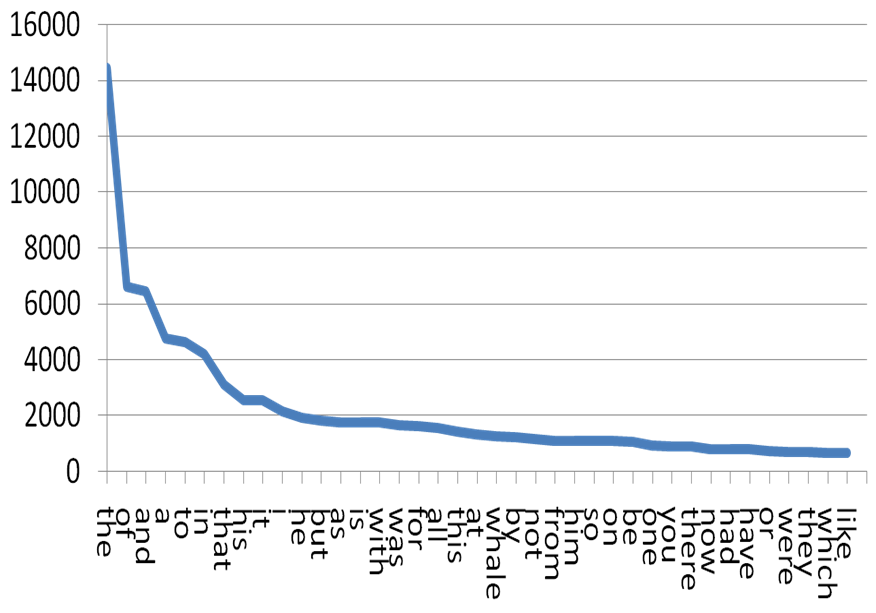
\includegraphics[scale=0.5]{pics/zipf1.png}
\end{figure}
\begin{itemize}
 \item Listar las palabras más frecuentes de un corpus se puede utilizar para construir una lista de \emph{stopwords}. 
\end{itemize}
\end{frame}

\begin{frame}\frametitle{Ley de Zipf (4/4)}
\begin{figure}[h!]
	\centering
	\includegraphics[scale=0.4]{pics/zipf_30wiki_es_labels.png}
\end{figure}
Si graficamos un gráfico $log$-$log$, obtenemos una línea recta con pendiente $-\beta$.
\end{frame}

\begin{frame}\frametitle{Representación Vectorial de Texto (1/2)}
\begin{itemize}
 \item El procesamiento de texto requiere convertir las palabras en números para poder realizar cálculos matemáticos.
 \item La representación vectorial permite:
   \begin{itemize}
     \item Calcular similitudes entre documentos
     \item Agrupar documentos similares
     \item Clasificar documentos
     \item Encontrar documentos relevantes para una consulta
    \end{itemize}
\end{itemize}
\end{frame}

\begin{frame}\frametitle{Representación Vectorial de Texto (2/2)}
  \begin{itemize}
   \item Una forma básica consiste en \textit{representar} los documentos como vectores de términos, donde cada término es una dimensión vectorial \cite{salton1975vector}.
   \item Documentos con diferentes palabras y longitudes residirán en el mismo espacio vectorial.
   \item A continuación veremos dos técnicas comunes para representar documentos como vectores: \emph{Bag of Words} y \emph{TF-IDF}.
\end{itemize}
\end{frame}

\begin{frame}\frametitle{Bag of Words (1/3)}
  \begin{itemize}
    \item La representación más simple y común de texto como vector es el modelo \emph{Bag of Words} (BoW).
    \item En BoW, un documento se representa como una ``bolsa'' (multiconjunto) de sus palabras.
    \item Características principales:
  \end{itemize}
  
  \hfill
  \begin{tabular}{|p{5cm}|p{5cm}|}
    \hline
    \textbf{Lo que ignora} & \textbf{Lo que considera} \\
    \hline
    Orden de las palabras & Frecuencia de cada palabra \\
    Estructura gramatical & Presencia/ausencia de términos \\
    Sintaxis & Distribución estadística \\
    \hline
  \end{tabular}
  \hfill
  \end{frame}

\begin{frame}\frametitle{Bag of Words (2/3)}
\begin{itemize}
   \item El valor de cada dimensión es un peso que representa la relevancia del término $t_{i}$ en el documento $d$:
   \begin{equation}
    d_{j} \rightarrow \overrightarrow{d_{j}}=(w(t_{1},d_{j}),...,w(t_{|V|},d_{j}))
   \end{equation}
\end{itemize}

\begin{block}{Ejemplo}
   Texto original: ``El gato come pescado y el perro come carne''
   
   Representación BoW:
   \begin{table}[h]
    \centering
    \small
    \renewcommand{\arraystretch}{0.8}
    \begin{tabular}{|l|c|}
    \hline
    \textbf{Término} & \textbf{Frecuencia} \\
    \hline
    el     & 2 \\
    gato   & 1 \\
    come   & 2 \\
    pescado& 1 \\
    y      & 1 \\
    perro  & 1 \\
    carne  & 1 \\
    \hline
    \end{tabular}
    \end{table}
\end{block}
\end{frame}

\begin{frame}\frametitle{Bag of Words (3/3)}
  \hfill
  \begin{table}[h]
    \centering
    \small 
    \begin{tabular}{|p{5cm}|p{5cm}|}
    \hline
    \textbf{Ventajas} & \textbf{Desventajas} \\
    \hline
    Simple de implementar & Pierde información contextual \\
    Computacionalmente eficiente & No captura la semántica \\
    Funciona para tareas básicas & No maneja bien negaciones \\
    Fácil de escalar & Alta dimensionalidad \\
    \hline
    \end{tabular}
    \end{table}
    \hfill

\begin{itemize}
\item A pesar de sus limitaciones, BoW es una representación fundamental que sirve como base para modelos más sofisticados.
\item Es especialmente útil en tareas como:
  \begin{itemize}
  \item Clasificación de documentos
  \item Recuperación de información
  \item Análisis de sentimientos básico
  \end{itemize}
\end{itemize}
\end{frame}

\begin{frame}\frametitle{Term Frequency - Inverse Document Frequency (TF-IDF)}
\begin{itemize}
    \item TF-IDF es una medida estadística que evalúa qué tan relevante es una palabra para un documento en una colección
    \item Combina dos métricas:
    \begin{itemize}
        \item \textbf{Term Frequency (TF)}: Frecuencia de la palabra en el documento
        \item \textbf{Inverse Document Frequency (IDF)}: Qué tan única es la palabra en toda la colección
    \end{itemize}
    \item Intuición:
    \begin{itemize}
        \item Si una palabra aparece mucho en un documento, probablemente sea importante (TF alto)
        \item Si una palabra aparece en pocos documentos, probablemente sea más distintiva (IDF alto)
    \end{itemize}
\end{itemize}
\end{frame}

\begin{frame}\frametitle{Term Frequency (TF)}
\begin{itemize}
    \item Term Frequency mide la frecuencia de un término en un documento
    \item Existen diferentes formas de calcular TF:
\end{itemize}

\begin{table}[h]
\centering
\begin{tabular}{|l|l|}
\hline
\textbf{Variante} & \textbf{Fórmula} \\
\hline
Frecuencia Cruda & $tf_{i,j} = f_{i,j}$ \\
\hline
Frecuencia Binaria & $tf_{i,j} = \begin{cases} 1 & \text{si } f_{i,j} > 0 \\ 0 & \text{caso contrario} \end{cases}$ \\
\hline
Frecuencia Logarítmica & $tf_{i,j} = 1 + \log(f_{i,j})$ \\
\hline
Frecuencia Normalizada & $tf_{i,j} = \frac{f_{i,j}}{\max_k f_{k,j}}$ \\
\hline
\end{tabular}
\end{table}

Donde $f_{i,j}$ es la frecuencia del término $i$ en el documento $j$
\end{frame}

\begin{frame}\frametitle{Inverse Document Frequency (IDF)}
\begin{itemize}
    \item IDF mide qué tan común o raro es un término en toda la colección
    \item Penaliza términos que aparecen en muchos documentos
    \item Fórmula básica:
    \[ idf_i = \log\left(\frac{N}{n_i}\right) \]
    \begin{itemize}
        \item $N$ = número total de documentos
        \item $n_i$ = número de documentos que contienen el término $i$
    \end{itemize}
\end{itemize}

\begin{table}[h]
  \small
  \centering
\begin{tabular}{|l|c|c|c|}
\hline
\textbf{Término} & \textbf{Docs con término} & \textbf{Total docs} & \textbf{IDF} \\
\hline
"el" & 98 & 100 & 0.02 \\
"algoritmo" & 5 & 100 & 3.00 \\
"pelotillehue" & 1 & 100 & 4.61 \\
\hline
\end{tabular}
\end{table}

\begin{itemize}
    \item Palabras comunes como ``el'' tienen IDF bajo y palabras raras como ``pelotillehue'' tienen IDF alto
\end{itemize}
\end{frame}

\begin{frame}\frametitle{Cálculo Final de TF-IDF (1/2)}
\begin{itemize}
    \item El peso final TF-IDF se calcula multiplicando TF × IDF:
    \[ w_{i,j} = tf_{i,j} \times idf_i \]
\end{itemize}

\begin{block}{Ejemplo}
\vspace{0.5em}
  Documento: ``El gato come pescado. El gato duerme''
\begin{table}[h]
\centering
\begin{tabular}{|l|c|c|c|c|}
\hline
\textbf{Término} & \textbf{TF} & \textbf{IDF} & \textbf{TF-IDF} & \textbf{Interpretación} \\
\hline
"el" & 2 & 0.02 & 0.04 & Poco relevante \\
"gato" & 2 & 2.30 & 4.60 & Muy relevante \\
"come" & 1 & 2.70 & 2.70 & Relevante \\
"pescado" & 1 & 3.00 & 3.00 & Relevante \\
"duerme" & 1 & 2.70 & 2.70 & Relevante \\
\hline
\end{tabular}
\end{table}
\end{block}
\end{frame}

\begin{frame}\frametitle{Cálculo Final de TF-IDF (2/2)}
\begin{itemize}
    \item Las palabras con alto TF-IDF son las más características del documento
    \item Este peso se usa para construir los vectores de documentos
    \item Propiedades importantes del TF-IDF:
    \begin{itemize}
        \item Asigna mayor peso a términos frecuentes en pocos documentos
        \item Penaliza términos que aparecen en muchos documentos
        \item Es independiente del tamaño del documento
        \item Facilita la comparación entre documentos
    \end{itemize}
\end{itemize}
\end{frame}

\begin{frame}\frametitle{Similitud entre Vectores (1/2)}
\begin{itemize}
 \item Representar consultas y documentos como vectores permite calcular su similitud.
 \item Un enfoque sería usar la distancia euclidiana.
 \item El enfoque común es calcular el coseno del ángulo entre los dos vectores.
 \item Si ambos documentos son iguales:
   \begin{itemize}
     \item El ángulo sería $0$ 
     \item Su coseno sería $1$
   \end{itemize}
 \item Si los documentos son ortogonales:
   \begin{itemize}
     \item El coseno es $0$
   \end{itemize}
\end{itemize}
\end{frame}

\begin{frame}\frametitle{Similitud entre Vectores (2/2)}
\begin{itemize}
 \item La similitud del coseno se calcula de la siguiente manera:
 \begin{displaymath}
 cos(\vec{d}_{1},\vec{d}_{2})= \frac{\vec{d}_{1}\cdot \vec{d}_{2}}{|\vec{d}_{1}|\times|\vec{d}_{2}|} = \frac{\sum_{i=1}^{|V|}(w(t_{i},d_{1})\times w(t_{i},d_{2}))}{\sqrt{\sum_{i=1}^{|V|} w(t_{i},d_{1})^2}\times \sqrt{\sum_{i=1}^{|V|} w(t_{i},d_{2})^2}}
 \end{displaymath}
 \item Esto se llama erróneamente \emph{distancia del coseno}. En realidad, es una métrica de similitud.
 \item Tenga en cuenta que la similitud del coseno normaliza los vectores por su norma euclidiana $||\vec{d}||_{2}$.
\end{itemize}
\end{frame}

\begin{frame}{Similitud del Coseno}

\begin{figure}[h!]
	\centering
	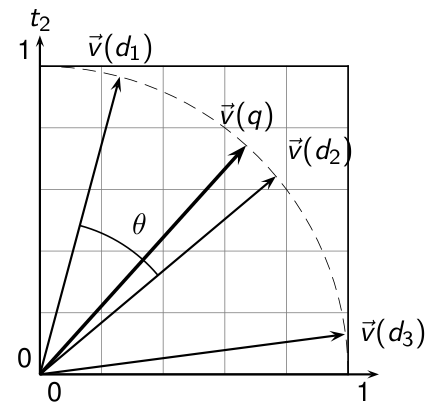
\includegraphics[scale=0.5]{pics/cos.png}
	\caption{ Similitud del Coseno.}
\end{figure}

\end{frame}

\begin{frame}{Ejercicio}
\begin{itemize}
 \item Supongamos que tenemos $3$ documentos formados a partir de las siguientes secuencias de términos: \\
 $d_{1}\rightarrow t_{4}t_{3}t_{1}t_{4}$ \\
 $d_{2}\rightarrow t_{5}t_{4}t_{2}t_{3}t_{5}$ \\
 $d_{3}\rightarrow t_{2}t_{1}t_{4}t_{4}$ \\

\item Construya una matriz de términos-documentos de $5\times3$ dimensiones usando pesos $tf$-$idf$ simples (sin normalización).
\item  Le recomendamos que primero construya una lista con el número de documentos en los que aparece cada término (útil para calcular las puntuaciones $idf$)
\item Luego calcule las puntuaciones $idf$ de cada término.
\item Llene las celdas de la matriz con los valores $tf$-$idf$.
\item ¿Cuál es el documento más cercano a $d_{1}$?
\end{itemize}


\end{frame}

\begin{frame}{Resultado}
 \begin{table}[htbp]
\caption{Matriz tf-idf}
\begin{tabular}{|l|r|r|r|}
\hline
 & \multicolumn{1}{l|}{d1} & \multicolumn{1}{l|}{d2} & \multicolumn{1}{l|}{d3} \\ \hline
t1 & 0.176 & 0.000 & 0.176 \\ \hline
t2 & 0.000 & 0.176 & 0.176 \\ \hline
t3 & 0.176 & 0.176 & 0.000 \\ \hline
t4 & 0.000 & 0.000 & 0.000 \\ \hline
t5 & 0.000 & 0.954 & 0.000 \\ \hline
\end{tabular}
\end{table}

\end{frame}

\begin{frame}\frametitle{N-gramas (1/2)}
\begin{itemize}
 \item Los n-gramas son secuencias contiguas de n elementos (palabras o caracteres).
 \item Tipos comunes:
   \begin{itemize}
     \item Unigramas (n=1): palabras individuales
     \item Bigramas (n=2): pares de palabras consecutivas
     \item Trigramas (n=3): tríos de palabras consecutivas
   \end{itemize}
 \item Aplicaciones en BoW y TF-IDF:
   \begin{itemize}
     \item Se pueden usar como términos en vez de palabras individuales
     \item Permiten capturar frases y expresiones completas
     \item Mejoran la precisión en búsquedas de frases exactas
   \end{itemize}
 \item Desventajas:
   \begin{itemize}
    \item Mayor dispersión de los vectores
    \item Mayor costo computacional
   \end{itemize}
\end{itemize}
\end{frame}

\begin{frame}\frametitle{N-gramas (2/2)}
\begin{block}{Ejemplo}
  \vspace{0.5em}
  \texttt{``El gato negro duerme'' }
    \begin{itemize}
     \item Unigramas: \texttt{[el] [gato] [negro] [duerme]}
     \item Bigramas: \texttt{[el gato] [gato negro] [negro duerme]}
     \item Trigramas: \texttt{[el gato negro] [gato negro duerme]}
    \end{itemize}
\end{block}

\begin{itemize}
 \item En BoW/TF-IDF con n-gramas:
   \begin{itemize}
     \item Cada n-grama es una dimensión independiente
     \item Se pueden combinar diferentes valores de n
     \item Se suele usar n ≤ 3 por razones prácticas
   \end{itemize}
\end{itemize}
\end{frame}

\begin{frame}\frametitle{Conceptos Adicionales}
\begin{itemize}
 \item Los sistemas modernos de recuperación de información van más allá de la similitud vectorial:
   \begin{itemize}
     \item PageRank
     \item Relevance Feedback
     \item Query log mining
     \item Google Knowledge Graph
     \item Machine Learning
   \end{itemize}
 \item La recuperación de información y la minería de textos están menos preocupadas por la estructura lingüística y más interesadas en producir algoritmos rápidos y escalables \cite{jacobbook}.
\end{itemize}
\end{frame}

\begin{frame}\frametitle{Conclusiones}
\begin{itemize}
 \item Representar documentos como vectores sirve para calcular similitudes entre pares de documentos.
 \item Los vectores Bag of words y TF-IDF son dos representaciones que:
   \begin{itemize}
     \item Carecen de estructura lingüística
     \item Son de alta dimensión y dispersos
     \item Pueden mejorarse con n-gramas para capturar expresiones multipalabra
   \end{itemize}
\end{itemize}
\end{frame}

\begin{frame}[allowframebreaks]\scriptsize
\frametitle{Referencias}
\bibliography{bio}
\bibliographystyle{apalike}
%\bibliographystyle{flexbib}
\end{frame}



%%%%%%%%%%%%%%%%%%%%%%%%%%%

\end{document}
